% Standalone RAKL claim / authority-ledger lifecycle diagram (Paper I).
% Build:  pdflatex claim_lifecycle.tex  -> claim_lifecycle.pdf
\documentclass[border=6pt]{standalone}
\usepackage{tikz}
\usepackage{helvet}\renewcommand{\familydefault}{\sfdefault}
\usetikzlibrary{positioning,arrows.meta,fit,backgrounds,calc}
\begin{document}
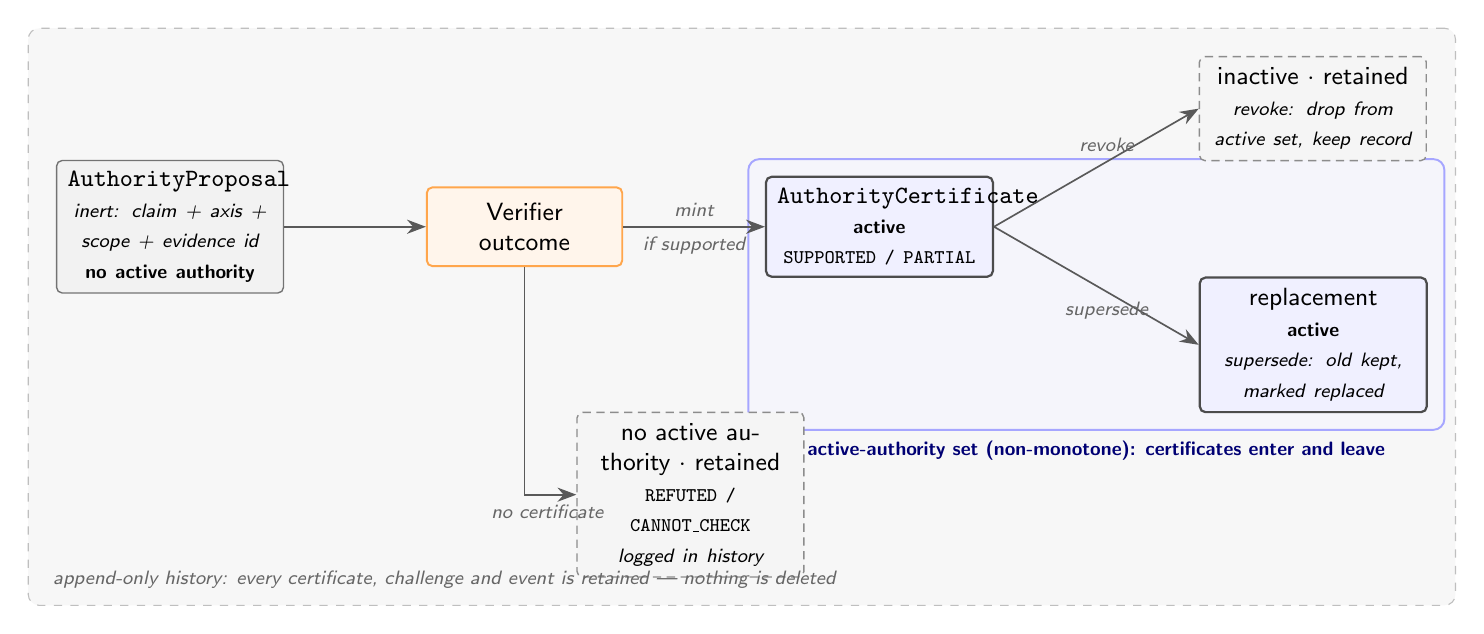
\begin{tikzpicture}[
  font=\small,
  >={Stealth[length=2.4mm]},
  st/.style={rounded corners=2pt, draw=black!55, line width=0.5pt, align=center,
             inner sep=4pt, minimum height=10mm, text width=26mm, fill=white},
  inert/.style={st, fill=black!5},
  active/.style={st, draw=black!70, line width=0.8pt, fill=blue!6},
  retain/.style={st, fill=black!4, draw=black!45, dash pattern=on 3pt off 2pt},
  flow/.style={->, line width=0.6pt, draw=black!65},
  lbl/.style={font=\scriptsize\itshape, text=black!60},
  node distance=9mm and 18mm,
]
% ---- proposal (inert, no authority) ----
\node[inert] (prop) {\texttt{AuthorityProposal}\\{\scriptsize\itshape inert: claim + axis +}\\{\scriptsize\itshape scope + evidence id}\\{\scriptsize\bfseries no active authority}};

% ---- verifier gate ----
\node[st, right=of prop, fill=orange!8, draw=orange!70, line width=0.7pt, text width=22mm]
  (ver) {Verifier\\outcome};

% ---- active certificate (supported / partial) ----
\node[active, right=of ver] (cert)
  {\texttt{AuthorityCertificate}\\{\scriptsize\bfseries active}\\{\scriptsize\ttfamily SUPPORTED / PARTIAL}};

% ---- terminal retained states (top: revoke, mid: supersede, bottom: refuted) ----
\node[retain, right=26mm of cert, yshift=15mm] (revoked)
  {inactive $\cdot$ retained\\{\scriptsize\itshape revoke: drop from}\\{\scriptsize\itshape active set, keep record}};
\node[active, right=26mm of cert, yshift=-15mm] (super)
  {replacement\\{\scriptsize\bfseries active}\\{\scriptsize\itshape supersede: old kept,}\\{\scriptsize\itshape marked replaced}};
\node[retain, below=17mm of cert, xshift=-24mm] (refuted)
  {no active authority $\cdot$ retained\\{\scriptsize\ttfamily REFUTED / CANNOT\_CHECK}\\{\scriptsize\itshape logged in history}};

% ---- flows ----
\draw[flow] (prop) -- (ver);
\draw[flow] (ver) -- node[lbl,above]{mint}
                     node[lbl,below]{if supported} (cert);
\draw[flow] (cert.east) -- node[lbl,above,pos=0.55]{revoke} (revoked.west);
\draw[flow] (cert.east) -- node[lbl,below,pos=0.55]{supersede} (super.west);
\draw[flow] (ver.south) |- node[lbl,below,pos=0.72]{no certificate} (refuted.west);

% ---- append-only history band (contains everything: nothing deleted) ----
\begin{scope}[on background layer]
  \node[draw=black!25, dashed, rounded corners=4pt, fill=black!3,
        fit=(prop)(ver)(cert)(revoked)(super)(refuted), inner sep=10pt] (hist) {};
\end{scope}
\node[lbl, anchor=south west] at ($(hist.south west)+(2mm,1mm)$)
  {append-only history: every certificate, challenge and event is retained --- nothing is deleted};

% ---- active-set overlay (non-monotone: certificates enter and leave) ----
\begin{scope}[on background layer]
  \node[draw=blue!35, rounded corners=4pt, line width=0.7pt, fill=blue!4, fill opacity=0.5,
        fit=(cert)(super), inner sep=6pt] (act) {};
\end{scope}
\node[font=\scriptsize\bfseries, text=blue!45!black, anchor=north]
  at (act.south) {active-authority set (non-monotone): certificates enter and leave};
\end{tikzpicture}
\end{document}
